\chapter{Los números complejos}
$(\mathbb{R}^2, +, \cdot)$ con las siguientes operaciones
\begin{itemize}
    \item Suma : $(a,b) + (c,d) = (a + b, c + d)$.
    \item Producto: $(a,b) \cdot (c,d) = (ac - bd, ad + bc)$
\end{itemize}
es un cuerpo, lo llamaremos $\mathbb{C}$ y sus elementos se llaman números complejos.

Observamos que
\begin{align*}
    E = \{ (a,0) : a \in \mathbb{R} \} \subset \mathbb{C}
\end{align*}
es subcuerpo de $\mathbb{C}$, pues
\begin{itemize}
    \item $(a,0) + (c,0) = (a+c,0) \in E$.
    \item $(a,0) \cdot (c,0) = (ac,0) \in E$.
    \item El opuesto de $(a,0)$ es $(-a,0) \in E$.
    \item El inverso de $(a,0) \not = (0,0)$ es $\left(\frac{1}{a},0\right) \in E$.
\end{itemize}
Esto nos dice que $E$ es subcuerpo de $\mathbb{C}$. Además $E$ es isomorfo a $\mathbb{R}$ (en sentido de cuerpos) mediante la siguiente identificación
\begin{align*}
    (a,0) \in E \longleftrightarrow a \in \mathbb{R}
\end{align*}
\section{Terminología y nomenclatura}
\begin{enumerate}
    \item[1)] Los elementos de $\mathbb{C} \longleftrightarrow \mathbb{R}^2$ se llaman números complejos.
    \item[2)] Si $(a,b) \in \mathbb{C}$, su parte real es $a$ y su parte imaginaria es $b$.
    \item[3)] $(1,0) \equiv 1$.
    \item[4)] $(0,1) \equiv i$.
\end{enumerate}
Mediante la identificación $E \longleftrightarrow \mathbb{R}$, tenemos que para $x,y \in \mathbb{R}$
\begin{itemize}
    \item $x \cdot 1 = x$.
    \item $y \cdot i = (0,y)$.
    \item $(x,y) = (x,0) + (0,y) = x + iy$.
\end{itemize}
De esta manera
\begin{align*}
    \mathbb{C} = \{ x + iy : x,y \in \mathbb{R} \}.
\end{align*}
Los números complejos se representan en $\mathbb{R}^2$ de la siguiente manera:

\begin{align*}
    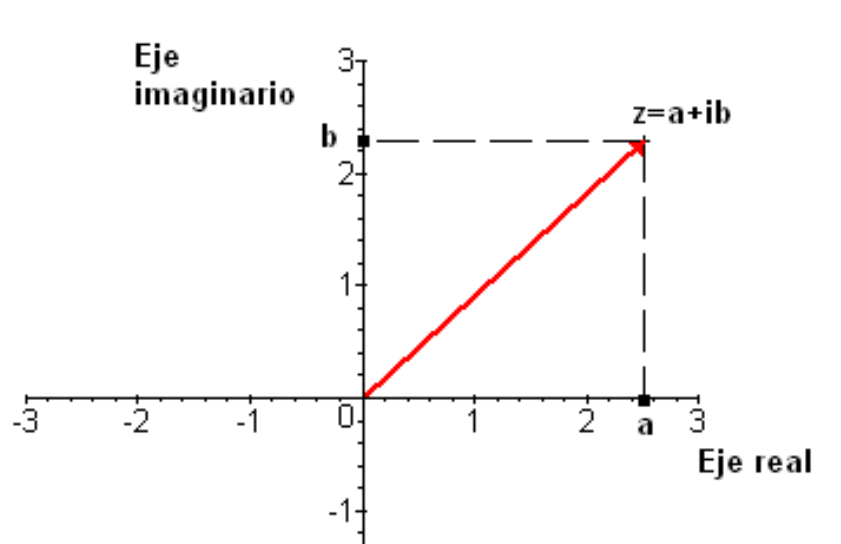
\includegraphics[width=0.4\textwidth]{imagenes/complejos.png}
\end{align*}

Si $z = x + iy \in \mathbb{C}$, entonces $\re(z) = x$ e $\im(z) = y$.
\begin{itemize}
    \item $\mathbb{C}$ no tiene orden ($\mathbb{R}$ sí).
    \item $i^2 = (0,1) \cdot (0,1) = (-1,0) = -1$.
\end{itemize}

\begin{defi}
    Si $z = a + ib \in \com$, definimos su conjugado como $\overline{z} = a - ib$.
\end{defi}

Esta operación de conjugación se puede ver en $\mathbb{R}^2$ como la siguiente aplicación lineal

\begin{align*}
    \mathbb{R}^2    & \longrightarrow \mathbb{R}^2           \\
    \begin{pmatrix}
        x \\
        y
    \end{pmatrix} & \longmapsto \begin{pmatrix}
                                    1 & 0  \\
                                    0 & -1
                                \end{pmatrix} \begin{pmatrix}
                                                  x \\
                                                  y
                                              \end{pmatrix}
\end{align*}

Algunas propiedades innmediatas son
\begin{enumerate}
    \item[1)] $\overline{0} = 0$.
    \item[2)] $\overline{1} = 1$.
    \item[3)] $\overline{z + w} = \overline{z} + \overline{w}$, $z,w \in \com$.
    \item[4)] $\overline{z \cdot w} = \overline{z} \cdot \overline{w}$, $z,w \in \com$.
    \item[5)] Involución : $\overline{\overline{z}} = z$, $z \in \com$.
    \item[6)] Si $z = a + ib \in \com$,
          \begin{align*}
              \re(z) = a = \frac{z + \overline{z}}{2} \ \ \ \text{y} \ \ \ \im(z) = b = \frac{z - \overline{z}}{2i}.
          \end{align*}
\end{enumerate}

\section{$\mathbb{C}$ como espacio vectorial}
Al estar $\mathbb{C}$ identificado con $\mathbb{R}^2$, tenemos que $\mathbb{C}$ es un espacio vectorial de dimensión 2. La base canónica es $\{1,i\}$. Pero como $\mathbb{C}$ es un cuerpo, tenemos que es un espacio vectorial complejo de dimensión y tiene como base canónica $\{1\}$.

Veamos como son las aplicaciones lineales de $\mathbb{C}$ en $\mathbb{C}$.
\begin{itemize}
    \item \textbf{Punto de vista real}.
          \begin{align*}
              L : \com        & \longrightarrow \com                     \\
              \begin{pmatrix}
                  x \\
                  y
              \end{pmatrix} & \longmapsto L\begin{pmatrix}
                                               x \\
                                               y
                                           \end{pmatrix} = xL(1) + yL(i)
          \end{align*}
          En términos de números complejos, $z = x + iy$. Entonces
          \begin{align*}
              L(z) & = L \begin{pmatrix}
                             x \\
                             y
                         \end{pmatrix} = \begin{pmatrix}
                                             a_{11} & a_{12} \\
                                             a_{21} & a_{22}
                                         \end{pmatrix} \begin{pmatrix}
                                                           x \\
                                                           y
                                                       \end{pmatrix}                                                                   \\
                   & =                                                                                                                  \\
                   & \ \vdots                                                                                                           \\
                   & = \frac{(a_{11} + a_{22}) + i(-a_{12} + a_{21})}{2}z + \frac{(a_{11} - a_{22}) +i(a_{12} + a_{21})}{2}\overline{z} \\
                   & = \alpha z + \beta \overline{z}.
          \end{align*}
    \item \textbf{Punto de vista complejo}
          \begin{align*}
              L : \com & \longrightarrow \com \\
              z        & \longmapsto zL(1)
          \end{align*}
\end{itemize}

Veamos como son las \textbf{rectas de números complejos}. En $\mathbb{R}$ una recta es de la forma
\begin{align*}
    Ax + By + C = 0, \ \ \ A,B,C \in \mathbb{R}, |A| + |B| > 0.
\end{align*}
En términos de números complejos
\begin{align*}
    0 & = A \frac{z + \overline{z}}{2} + B \frac{z - \overline{z}}{2i} + C = \frac{A - iB}{2}z + \frac{A +iB}{2}\overline{z} + C \\
      & = \beta z + \overline{\beta}\overline{z} + \gamma \ \ \text{donde } \beta = \frac{A - iB}{2}, \gamma = C.
\end{align*}
Nos queda que la ecuación de una recta en el plano complejo es
\begin{align*}
    \boxed{
        (E) \ \beta z + \overline{\beta}\overline{z} + \gamma = 0, \ \ \ \beta \in \com, \beta \not = 0, \gamma \in \mathbb{R}
    }
\end{align*}

\begin{defi}
    Definimos el módulo o valor absoluto de un número complejo como la aplicación
    \begin{align*}
        |.| : \com & \longrightarrow\mathbb{R}^+                                           \\
        z          & \longmapsto \sqrt{\re(z)^2 + \im(z)^2} = \sqrt{z \cdot \overline{z}}.
    \end{align*}
\end{defi}
Veamos que el módulo es, efectivamente, una norma.
\begin{proof}
    \begin{enumerate}
        \item $|z| \ge 0$.
        \item $|z| = 0 \Longleftrightarrow z = 0$.
        \item Desigualdad triangular : $|z + w| \leq |z| + |w|$. Veamoslo. Sean $z = x + iy$, $w = u +iv$ donde $x,y,u,v \in \mathbb{R}$.

              \textit{Cuentas previas}
              \begin{enumerate}
                  \item[(i)]
                        \begin{align*}
                            \re(z) & = x \leq |x| = \sqrt{x^2} \leq \sqrt{x^2 + y^2} = |z|  \\
                            \im(z) & = y \leq |y| = \sqrt{y^2} \leq \sqrt{x^2 + y^2} = |z|.
                        \end{align*}
                  \item[(ii)] $|z \cdot w| = \sqrt{(zw) \cdot \overline{(zw)}} = \sqrt{z\overline{z}w\overline{w}} = \sqrt{|z|^2|w|^2} = |z|\cdot |w|$.
                  \item[(iii)] $|\overline{z}| = |z|$.
              \end{enumerate}
              Ahora si, pasamos a probar la desigualdad triangular.
              \begin{align*}
                  |z+w|^2 & = (z+w)\overline{(zw)} = z\overline{z} + w\overline{w} + z\overline{w} + \overline{z}w \\
                          & = |z|^2 + |w|^2 + 2\re(z\overline{w})                                                  \\
                          & \leq |z|^2 + |w|^2 + 2|z\overline{w}| = |z|^2 + |w|^2 + 2|z||\overline{w}|             \\
                          & = |z|^2 + |w|^2 + 2|z||w|                                                              \\
                          & = (|z| + |w|)^2
              \end{align*}
              Luego $|z+w| \leq |z| + |w|$.
        \item Compatibilidad de la norma con el producto por escalares.
              \begin{align*}
                  |\lambda z| = |\lambda| |z|, \ \ \ \lambda, z \in \com.
              \end{align*}
    \end{enumerate}
\end{proof}
El hecho de tener definida la multiplicación en $\com$ y la propiedad $|zw| = |z||w|$ nos dice que $\com$ es un álgebra (real o compleja) conmutativa (por ser la multiplicación conmutativa). La norma que hemos defiindo en $\com$ viene del siguiente producto escalar complejo
\begin{align*}
    <.,.> : \com \times \com & \longrightarrow \com                     \\
    (z,w)                    & \longmapsto <z,w>_{\com} = z\overline{w}
\end{align*}
Veamos que es, efectivamente, un producto escalar complejo
\begin{proof}
    \begin{enumerate}
        \item Sesguilinealidad (lineal por la izquierda y lineal conjugado por la derecha). Dados $\lambda_1, \lambda_2 \in \com$, $z,z_2,z_2,w,w_1,w_2 \in \com$ entonces
              \begin{align*}
                  <\lambda_1z_2 + \lambda_2z_2,w>_{\com} & = \lambda_1<z_1,w>_{\com} + \lambda_2<z_2,w>_{\com}                       \\
                  <z,\lambda_2w_2 + \lambda_2w_2>_{\com} & = \overline{\lambda_1}<z,w_1>_{\com} + \overline{\lambda_2}<z,w_2>_{\com}
              \end{align*}
        \item Hermeticidad (simetría conjugada). Dados $z,w \in \com$ entonces
              \begin{align*}
                  <z,w>_{\com} = z\overline{w} = \overline{\overline{z\overline{w}}} = \overline{\overline{z}w} = \overline{w\overline{z}} = \overline{<w,z>_{\com}}
              \end{align*}
        \item Definido positivo. Dado $z \in \com$. Entonces
              \begin{align*}
                   & <z,z>_{\com} = z\overline{z} = |z|^2 \ge 0 \ \ \ \text{y}                 \\
                   & <z,z>_{\com} = 0 \Longleftrightarrow |z|^2 = 0 \Longleftrightarrow z = 0.
              \end{align*}
    \end{enumerate}
\end{proof}
Podemos ver este producto escalar en $\mathbb{R}^2$ en términos complejos. Sean
\begin{align*}
    z_1 = x_1 + iy_1 \text{ \ \ \ y \ \ \ } z_2 = x_2 + iy_2,
\end{align*}
$x_1,y_1,x_2,y_2 \in \mathbb{R}$. Entonces
\begin{align*}
    <(x_1,y_1), (x_2,y_2)>_{\mathbb{R}^2} = x_1x_2 + y_1y_2 = \re(z_1\overline{z_2}).
\end{align*}
Veamos como es una \textbf{circunferencia de números complejos} de centro $z_0 = x_0 +iy_0$ y radio $r > 0$.
\begin{align*}
    (E) \ \{ z \in \com : |z - z_0| = r \}
\end{align*}
\begin{align*}
    0 & = |z-z_0|^2 - r^2 = ... = |z|^2 + |z_0|^2 - 2\re(z\overline{z_0}) - r^2 \\
      & = |z|^2 - \overline{z_0}z - z_0\overline{z} + |z_0|^2 - r^2.
\end{align*}
Multiplicando por $\alpha \in \mathbb{R}$, $\alpha \not = 0$
\begin{align*}
    0 & = \alpha |z|^2 - \alpha \overline{z_0}z - \alpha z_0\overline{z} + \alpha (|z_0|^2 - r^2) \\
\end{align*}
Llamando $\beta = -\alpha\overline{z_0}z$ y $\gamma =  \alpha (|z_0|^2 - r^2)$ nos queda que
\begin{align*}
    \alpha|z|^2 + \beta z + \overline{\beta} \overline{z} + \gamma = 0
\end{align*}
donde $\alpha, \gamma \in \mathbb{R}$, $\alpha \not = 0$, $\beta \in \com$ y $|\beta|^2 > \alpha \gamma$. Si $\alpha = 0$ tendríamos la ecuación de una recta.

Nos queda que la ecuación de una circunferencia (o recta) en el plano complejo es
\begin{align*}
    \boxed{
        (E) \ \alpha|z|^2 + \beta z + \overline{\beta} \overline{z} + \gamma = 0, \ \ \ \alpha, \gamma \in \mathbb{R}, \beta \in \com, |\beta|^2 > \alpha \gamma
    }
\end{align*}

\section{Topología en $\com$}

La norma $|.|$ en $\com$ genera la siguiente métrica
\begin{align*}
    d(z_2,z_2) = |z_1 - z_2|, \ \ \ z_1,z_2 \in \com.
\end{align*}
Como sabemos, una métrica genera un topología. Las bolas las llamaremos discos.
\begin{defi}
    Definimos
    \begin{itemize}
        \item Disco abierto de centro $z_0$ y radio $r$
              \begin{align*}
                  \Delta(z_0,r) = \mathbb{D}(z_0,r) = \{z \in \com : |z - z_0| < r \}.
              \end{align*}
        \item Circunferencia de centro $z_0$ y radio $r$
              \begin{align*}
                  \partial \Delta(z_0,r) = \text{C}(z_0,r) = \{z \in \com : |z - z_0| =  r \}.
              \end{align*}
        \item Disco cerrado de centro $z_0$ y radio $r$
              \begin{align*}
                  \overline{\Delta(z_0,r)} = \{z \in \com : |z - z_0| \leq r \}.
              \end{align*}
    \end{itemize}
\end{defi}
Con la métrica inducida tenemos el concepto de convergencia de sucesiones y el concepto de continuidad.
\begin{obs}
    $(\com, |.|)$ es un espacio vectorial normado completo, es decir, toda sucesión de Cauchy converge. En cuanto a la continuidad de funciones, $f: D \subset \com \longrightarrow \com$ es continua si y solo si
    \begin{align*}
         & \re(f) : D \longrightarrow \mathbb{R} \text{ es continua y } \\
         & \im(f) : D \longrightarrow \mathbb{R} \text{ es continua}.
    \end{align*}
    Tenemos que $(\com, +, \cdot, |.|)$ es un álgebra de Banach conmutativa, luego la teoría de series de potencias tiene sentido completo en $\com$ y, en particular, podemos definir la exponencial de cualquier número complejo de la siguiente manera
    \begin{align*}
        e^z = \sum_{n=0}^{\infty}{\frac{z^n}{n!}}, \ \ z \in \com,
    \end{align*}
    y como el producto es conmutativo,
    \begin{align*}
        e^{z_1 + z_2} = e^{z_1} \cdot e^{z_2}, \ \ z_1,z_2 \in \com.
    \end{align*}
\end{obs}
Algunas propiedades de la exponencial son
\begin{enumerate}
    \item[1)] $e^0 = 1$.
    \item[2)] $e^x = \sum_{n=0}^{\infty}{\frac{x^n}{n!}}$, $x \in \mathbb{R}$.
    \item[3)] $z = x +iy$, $x,y \in \mathbb{R}$ entonces
          \begin{align*}
              e^z = e^{x+iy} = e^{x}e^{iy} = e^{x}\sum_{n=0}^{\infty}{\frac{(iy)^n}{n!}} = ... = e^{x}(\cos(y) + i\sen(y))
          \end{align*}
          \begin{itemize}
              \item $\re(e^z) = e^x\cos(y) = e^{\re(z)}\cos(\im(z))$.
              \item $\im(e^z) = e^x\sen(y) = e^{\re(z)}\sen(\im(z))$.

                    Al ser $\re(e^z)$ e $\im(e^z)$ continuas, se tiene que $e^z$ es continua en $\com$.
              \item $|e^z| = \sqrt{(e^x\cos(y))^2 + (e^x\sen(y))^2} = e^x$, donde $z = x + iy \in \com$. En particular $|e^{i\theta}| = 1$, para todo $\theta \in \mathbb{R}$.
              \item $\overline{e^z} = \overline{e^{x +iy}} = \overline{e^x(\cos(y) + i\sen(y))} = e^x(\cos(y) - i\sen(y)) = e^x(\cos(y) + i\sen(-y)) = e^{\overline{z}}$.
          \end{itemize}
    \item[4)] La exponencial compleja es periódica de periodo $2\pi i$.
          \begin{align*}
              e^{z + 2\pi i} & = e^{x + i(y + 2\pi)} = e^x(\cos(y + 2\pi) + i\sen(y + 2\pi)) \\
                             & = e^x(\cos(y) + i\sen(y)) = e^z.
          \end{align*}
          En particular, la exponencial no es inyectiva.
    \item[5)] La exponencial no es sobreyectiva, pues $e^z \not = 0$ para todo $z \in \com$. De hecho, el $0$ es el único número omitido por la exponencial, es decir, si $w \in \com \backslash \{0\}$, entonces existe $z \in \com$ tal que $e^z = w$.
\end{enumerate}

\section{Representación polar y exponencial de números complejos}

\begin{defi}
    Si $z \in \comz$, definimos el argumento de z como el siguiente conjunto
    \begin{align*}
        \arg(z) = \left\{ \theta \in \mathbb{R} : \cos(\theta) = \frac{\re(z)}{|z|}, \sen(\theta) = \frac{\im(z)}{|z|} \right\}
    \end{align*}
\end{defi}

\begin{prop}
    Si $\theta_0 \in \arg(z)$ entonces $\arg(z) = \{ \theta_0 + 2k\pi : k \in \mathbb{Z} \}$.
\end{prop}

\begin{proof}
    Solo hace falta probar que $\arg(z) \supseteq \{ \theta_0 + 2k\pi : k \in \mathbb{Z} \}$ (la otra inclusión es fácil de ver). Sea $\theta_1 \in \arg(z)$. Entonces
    \begin{align*}
        \cos(\theta_1) = \frac{\re(z)}{|z|} = \cos(\theta_0) \Longleftrightarrow \left\{ \begin{array}{lcc}
                                                                                             \theta_1 = \theta_0 + 2k\pi : k \in \mathbb{Z}  \\
                                                                                             \theta_1 = -\theta_0 + 2k\pi : k \in \mathbb{Z} \\
                                                                                         \end{array}
        \right.
    \end{align*}
    Si se da el primer caso, entonces se cumple la proposición. Supongamos que se da el segundo caso, entonces también ha de ocurrir que
    \begin{align*}
        \sen(\theta_1) = \frac{\im(z)}{|z|} = \sen(\theta_0)
    \end{align*}
    luego,
    \begin{align*}
        \sen(-\theta_0) = \sen(-\theta_0 + 2k\pi) = \sen(\theta_0) \Longrightarrow 2\sen(\theta_0) = 0 \Longrightarrow \theta_0 = k_1\pi, \  k_1 \in \mathbb{Z}.
    \end{align*}
    De aquí
    \begin{align*}
        \theta_1 & = -\theta_0 + 2k\pi = -k_1\pi + 2k\pi               \\
                 & = k_1\pi - 2k_1\pi + 2k\pi = k_1\pi + 2(k - k_1)\pi \\
                 & = \theta_0 + 2(k - k_1)\pi.
    \end{align*}
\end{proof}

\begin{defi}
    Si $z \in \comz$, su argumento principal es
    \begin{align*}
        \argp(z) = \arg(z) \cap [-\pi,\pi)
    \end{align*}
\end{defi}

\begin{ejemplo}
    \begin{itemize}
        \item $\argp(1) = 0$.
        \item $\argp(i) = \frac{\pi}{2}$.
        \item $\argp(-1) = -\pi$.
        \item $\argp(-i) = -\frac{\pi}{2}$.
    \end{itemize}
\end{ejemplo}

\begin{obs}
    Si $z \in \comz$
    \begin{align*}
        \argp(z) = \left\{ \begin{array}{lcc}
                               \arccos\left( \frac{\re(z)}{|z|}\right)  & si & \im(z) > 0    \\
                               -\arccos\left( \frac{\re(z)}{|z|}\right) & si & \im(z) \leq 0 \\
                           \end{array}
        \right.
    \end{align*}
    Luego, $\argp : \com \backslash (-\infty,0] \longrightarrow \mathbb{R}$ es continua en $\com \backslash (-\infty,0]$ y no se puede ser extendida de forma continua a $(-\infty,0]$.
\end{obs}

\begin{defi}[Forma polar y exponencial]
    Sea $z \in \comz$, entonces
    \begin{itemize}
        \item Forma polar: $z = |z|(\cos\theta + i\sen\theta)$.
        \item Forma exponencial: $z = |z|e^{i\theta}$.
    \end{itemize}
\end{defi}
La representación exponencial de un número complejo es muy útil, por ejemplo,
\begin{enumerate}
    \item[1)] Multiplicación de números complejos: Dados $z_1 = r_1e^{i\theta_1}$ y $z_1 = r_2e^{i\theta_2}$ tenemos que
          \begin{align*}
              z_1z_2 = r_1e^{i\theta_1}r_2e^{i\theta_2} = r_1r_2e^{i(\theta_1 + \theta_2)} = r_1r_2(\cos(\theta_1 + \theta_2) + i\sen(\theta_1 + \theta_2))
          \end{align*}
    \item[2)] Desarrollando el miembro izquierdo de 1) tenemos que
          \begin{align*}
              z_1z_2 & = r_1(\cos\theta_1 + i\sen\theta_1)r_2(\cos\theta_2 + i\sen\theta_2)                                                    \\
                     & = r_1r_2(\cos\theta_1\cos\theta_2 - \sen\theta_1\sen\theta_2) + i(\cos\theta_1\sen\theta_2 + \sen\theta_1\cos\theta_2).
          \end{align*}
          Con lo que llegamos a la fórmula de la suma de ángulos en el coseno y el seno.
    \item[3)] Fórmula de Moivre.
          \begin{align*}
              (\cos\theta + i\sen\theta)^n = (e^{i\theta})^n = e^{in\theta} = \cos(n\theta) +i\sen(n\theta).
          \end{align*}
    \item[4)] Podemos ver $re^{i\theta}$ como un número complejo en la circunferencia de centro 0 radio $r$ que forma un ángulo $\theta$ con el eje real positivo.
\end{enumerate}

\begin{ejemplo}
    \begin{itemize}
        \item $i = e^{i\frac{\pi}{2}}$.
        \item $3 = 3e^{i\cdot 0} = 3$.
        \item $-3i = 3e^{-i\frac{\pi}{2}} = 3e^{i\frac{3\pi}{2}}$.
    \end{itemize}
\end{ejemplo}

Volvamos a la exponencial.
\begin{enumerate}
    \item[1)] Sabemos que la exponencial tiene periodo $2\pi i$. Veamos que este es el periodo más pequeño, para ello, hemos de probar que $e^z = e^w$ si y solo si $z - w = 2k\pi i$, $k \in \mathbb{Z}$. Solo tenemos que probar que si $e^z = e^w$ entonces $z - w = 2k\pi i$, $k \in \mathbb{Z}$ (la otra implicación ya la vimos).
          \begin{proof}
              \begin{align*}
                  e^z = e^w \Longleftrightarrow e^{z-w} = 1.
              \end{align*}
              Escribimos $z -w = x + iy$, $x,y \in \mathbb{R}$. Entonces
              \begin{align*}
                  e^{z-w} = 1 & \Longleftrightarrow e^x(\cos y + i\sen y) = 1 \Longleftrightarrow \left\{ \begin{array}{lcc}
                                                                                                              e^x\cos y = 1 \\
                                                                                                              e^x\sen y = 0 \\
                                                                                                          \end{array}
                  \right. \underset{e^x > 0}{\Longleftrightarrow} \left\{ \begin{array}{lcc}
                                                                              e^x\cos y = 1 \\
                                                                              \sen y = 0    \\
                                                                          \end{array}
                  \right.                                                                                                   \\
                              & \Longleftrightarrow \left\{ \begin{array}{lcc}
                                                                e^x\cos y = 1                \\
                                                                y = k\pi, \ k \in \mathbb{Z} \\
                                                            \end{array}
                  \right. \Longleftrightarrow \left\{ \begin{array}{lcc}
                                                          e^x(-1)^k = 1                \\
                                                          y = k\pi, \ k \in \mathbb{Z} \\
                                                      \end{array}
                  \right. \Longleftrightarrow \left\{ \begin{array}{lcc}
                                                          e^x \cdot 1 = 1                               \\
                                                          y = k\pi, \ k \in \mathbb{Z}, \ k \text{ par} \\
                                                      \end{array}
                  \right.                                                                                                   \\
                              & \Longleftrightarrow \left\{ \begin{array}{lcc}
                                                                x  = 0                       \\
                                                                y = k\pi, \ k \in \mathbb{Z} \\
                                                            \end{array}
                  \right. \Longleftrightarrow z - w = 2k\pi i, \ k \in \mathbb{Z}
              \end{align*}
          \end{proof}
          \begin{obs}
              Esto nos dice que $f(z) = e^z$ es inyectiva en cualquier banda horizontal de altura $2\pi$, es decir, del tipo
              \begin{align*}
                  S_{y_0} = \{ x + iy \in \com : y \in [y_0, y_0 + 2\pi) \}.
              \end{align*}
          \end{obs}
    \item[2)] $0$ es el único valor omitido por $f(z) = e^z$.
          \begin{proof}
              Sea $w \in \comz$. Vamos a encontrar $z \in \com$ tal que $e^z = w$. Tomamos la representación exponencial $w = re^{i\theta}$, $r>0$, $\theta \in \mathbb{R}$. Basta tomar $x = \log r$ e $y = \theta$, así
              \begin{align*}
                  e^z = e^{x + iy} = e^xe^{iy} = e^{\log r}e^{i\theta} = re^{i\theta} = w.
              \end{align*}
          \end{proof}
\end{enumerate}

\begin{obs}
    Si $k \in \mathbb{Z}$ y $e^z = w$, entonces $e^{z + 2k\pi i} = w$.
\end{obs}

Introducimos ahora la definición de logaritmo complejo.
\begin{defi}
    Si $z \in \comz$, definimos el logaritmo complejo de z como
    \begin{align*}
        \log(z) & = \{ w \in \com : e^w = z \} \\
                & = \log |z| + i\arg(z).
    \end{align*}
    Y definimos el logaritmo principal como $\logp(z) = \log|z| + i\argp(z)$.
\end{defi}
Algunas propiedades del logaritmo son
\begin{enumerate}
    \item[1)] Si $z_1,z_2 \in \comz$, $z_1 = r_1e^{i\theta_1}$, $z_2 = r_2e^{i\theta_2}$, $r_1,r_2 > 0$, $\theta_1 \in \arg(z_1)$ y $\theta_2 \in \arg(z_2)$, entonces
          \begin{align*}
              \arg(z_1z_2) = \arg(r_1e^{i\theta_1}r_2e^{i\theta_2}) = \arg(r_1r_2e^{i(\theta_1 + \theta_2)}) = \arg(z_1) + \arg(z_2).
          \end{align*}
          Con esto probado, es claro que $\log(z_1z_2) = \log(z_1) + \log(z_2)$ (como conjuntos).
    \item[2)] $\argp(z_1z_2)$ no es necesariamente $\argp(z_1) + \argp(z_2)$, basta tomar $z_1 = z_2 = i$.
          \begin{align*}
              \argp(i \cdot i) = \argp(-1) = -\pi \not = \pi = \frac{\pi}{2} + \frac{\pi}{2} = \argp(i) + \argp(i)
          \end{align*}
    \item[3)] $\argp$ es continua en $\com \backslash (-\infty,0]$ y no admite extensión continua a un conjunto mayor.
\end{enumerate}

\begin{defi}
    \begin{itemize}
        \item Sea $A \subset \comz$, decimos que $\varphi : A \longrightarrow \mathbb{R}$ es una rama (continua) de $\arg(z)$ en $A$, si $\varphi$ es continua en $A$ y $\varphi(z) \in \arg(z)$ para cada $z \in A$.
        \item Sea $A \subset \com$ y sea $f: A \longrightarrow \com$ continua, decimos que $\varphi : A \longrightarrow \mathbb{R}$ es una rama (continua) de $\arg(f)$ en $A$, si $\varphi$ es continua en $A$ y $\varphi(z) \in \arg(f(z))$ para cada $z \in A$.
        \item Sea $A \subset \comz$, decimos que $\psi : A \longrightarrow \mathbb{R}$ es una rama (continua) de $\log(z)$ en $A$, si $\psi$ es continua en $A$ y $\psi(z) \in \log(z)$ para cada $z \in A$, o  equivalentemente, si $e^{\psi(z)} = z$ para todo $z \in A$.
        \item Sea $A \subset \com$ y sea $f: A \longrightarrow \com$ continua, decimos que $\psi : A \longrightarrow \mathbb{R}$ es una rama (continua) de $\arg(f)$ en $A$, si $\psi$ es continua en $A$ y $\psi(z) \in \log(f(z))$ para cada $z \in A$, o  equivalentemente, si $e^{\psi(z)} = f(z)$ para todo $z \in A$.
    \end{itemize}
\end{defi}

\begin{ejemplo}
    \begin{enumerate}
        \item[1)] $\argp$ es una rama del $\arg(z)$ en $\com \backslash (-\infty,0]$.
        \item[2)] $\logp$ es una rama del $\log(z)$ en $\com \backslash (-\infty,0]$.
        \item[3)] $\varphi_0(z) = \arg(z) \cap [0,2\pi)$, $z \in \comz$ es continua en $\comz$ y por tanto es una rama de $\arg(z)$ en $\com \backslash [0,+\infty)$.
              \begin{proof}
                  Observamos que $\varphi_0(z) = \pi + \argp(-z)$.
                  \begin{enumerate}
                      \item[(i)] $\varphi_0(z) \in \pi + [-\pi,\pi) = [0,2\pi)$.
                      \item[(ii)] $\varphi_0(z) \in \arg(z)$ pues
                            \begin{align*}
                                \cos(\varphi_0(z)) & = \cos(\pi + \argp(-z)) = -\cos(\argp(-z)) = -\frac{\re(-z)}{|z|} = \frac{\re(z)}{|z|}  \\
                                \sen(\varphi_0(z)) & = \sen(\pi + \argp(-z)) = -\sen(\argp(-z)) = -\frac{\im(-z)}{|z|} = \frac{\im(z)}{|z|}.
                            \end{align*}
                      \item[(iii)] $\varphi_0$ es continua en $\com \backslash [0,+\infty)$ si y solo si $\pi + \argp(z)$ es continua en $\com \backslash [0,+\infty)$ si y solo si $\argp(-z)$ es continua en $\com \backslash [0+\infty)$ si y solo si $-z \not \in (-\infty,0]$ si y solo si $z \not \in [0,+\infty)$ si y solo si $z \in \com \backslash [0,+\infty)$.
                      \item[(iv)] $\varphi_0$ no adite extensión continua a un conjunto mayor (pues $\argp$ no admite extensión continua a un conjunto mayor).
                  \end{enumerate}
              \end{proof}
        \item[4)] Si $\theta_0 \in \mathbb{R}$ fijo, la función $\varphi_{\theta_0}(z) = \arg(z) \cap [\theta_0, \theta_0 + 2\pi)$, $z \in \comz$ está bien definida y es continua en $\com \backslash \{re^{i\theta_0} : r \ge 0 \}$. Por tanto, $\varphi_{\theta_0}$ es una rama del $\arg(z)$ en
              \begin{align*}
                  S_{\theta_0} = \com \backslash \{ re^{i\theta_0} : r \ge 0 \}
              \end{align*}
              y además
              \begin{align*}
                  \varphi_{\theta_0}(z) = \theta_0 + \pi + e^{-i(\theta_0 + \pi)}z.
              \end{align*}
        \item[(5)] Si $\theta_0 \in \mathbb{R}$ fijo, la función $\psi_{\theta_0}(z) = \log|z| + i\varphi_{\theta_0}(z)$, $z \in \comz$ está bien definida y es continua en $\com \backslash \{re^{i\theta_0} : r \ge 0 \}$. Por tanto, $\psi_{\theta_0}$ es una rama de $\log(z)$ en
              \begin{align*}
                  S_{\theta_0} = \com \backslash \{ re^{i\theta_0} : r \ge 0 \}
              \end{align*}
              y además
              \begin{align*}
                  e^{\varphi_{\theta_0}(z)} = e^{\log|z| + i\varphi_{\theta_0}(z)} = |z|e^{i\varphi_{\theta_0}(z)} = z.
              \end{align*}
    \end{enumerate}
\end{ejemplo}

\begin{obs}
    Sea $\Omega \subset \comz$, $\varphi : \Omega \longrightarrow \mathbb{R}$ y $\psi : \Omega \longrightarrow \mathbb{R}$.
    \begin{enumerate}
        \item[1)] $\varphi$ es una rama del $\arg(z)$ en $\Omega$ si y solo si $\log|z| + i\varphi(z)$ es una rama del $\log(z)$ en $\Omega$.
        \item[2)] $\psi$ es una rama del $\log(z)$ en $\Omega$ si y solo si $\re(\psi(z))$ ($= \log|z|$) e $\im(\psi(z))$ son ramas del $\arg(z)$ en $\Omega$.
    \end{enumerate}
\end{obs}

\begin{prop}
    Sea $\Omega \subset \comz$ conexo,
    \begin{enumerate}
        \item[1)] Si $\varphi_1, \varphi_2$ son ramas de $\arg(z)$ en $\Omega$, entonces existe $k \in \mathbb{Z}$ tal que $\varphi_2(z) = \varphi_1(z) + 2k\pi$, $z \in \Omega$.
        \item[2)] Si $\psi_1, \psi_2$ son ramas de $\log(z)$ en $\Omega$, entonces existe $k \in \mathbb{Z}$ tal que $\psi_2(z) = \psi_1(z) + 2k\pi i$, $z \in \Omega$.
    \end{enumerate}
\end{prop}

\begin{proof}
    Probaremos solo 1). Para cada $z \in \Omega$, $\varphi_1(z), \varphi_2(z) \in \arg(z)$, luego existe $k(z) \in \mathbb{Z}$ tal que
    \begin{align*}
        \varphi_2(z) - \varphi_1(z) = 2k(z)\pi, \ \ z \in \Omega.
    \end{align*}
    Observaos que $\varphi_2 - \varphi_1$ es continua en $\Omega$, que es conexo, luego $(\varphi_2 - \varphi_1)(\Omega)$ es conexo y además es la imagen de un conjunto discreto, por tanto, se tiene que reducir (por continuidad) a un punto, es decir, existe $k \in \mathbb{Z}$ tal que
    \begin{align*}
        \varphi_2(z) - \varphi_1(z) = 2k\pi, \ \ z \in \Omega.
    \end{align*}
\end{proof}

\begin{prop}
    Sea $A$ un conjunto conexo y $ f: A \longrightarrow \com$ continua.
    \begin{enumerate}
        \item[1)] Si $\varphi_1,\varphi_2$ son ramas de $\arg(f)$ en $A$, entonces existe $k \in \mathbb{Z}$ tal que $\varphi_2(z) = \varphi_1(z) + 2k\pi$, $z \in A$.
        \item[2)] Si $\psi_1,\psi_2$ son ramas de $\log(f)$ en $A$, entonces existe $k \in \mathbb{Z}$ tal que $\psi_2(z) = \psi_1(z) + 2k\pi i$, $z \in A$.
    \end{enumerate}
\end{prop}

\begin{prop}
    En el plano complejo
    \begin{itemize}
        \item No existe rama de $\arg(z)$ en $\comz$.
        \item No existe rama de $\log(z)$ en $\comz$.
    \end{itemize}
    De forma general, si $\Omega \subset \comz$ contiene una circunferencia $C$ de centro $0$ y radio $r$, entonces no existe una rama de $\arg(z)$ en $\Omega$ ni una rama de $\log(z)$ en $\Omega$.
\end{prop}

\begin{proof}
    Basta demostrar que no hay una rama del $\arg(z)$ en $C$. Supongamos por reducción al absurdo que $\varphi: C \longrightarrow \mathbb{R}$ es una rama de $\arg(z)$ en $C$, entonces $\varphi$ es continua en $C$ y $\varphi(z) \in \arg(z)$ para todo $z \in C$.

    Observamos que $\argp(z)$ es rama del $\arg(z)$ en $C \backslash \{ -r \}$. Por la proposición anterior:
    \begin{align*}
        \argp(z) = \varphi(z) + 2k\pi, \ \ z \in C \backslash \{-r\}.
    \end{align*}
    Esto nos dice que como $\varphi$ adimite extensión continua a $C$, entonces $\argp(z)$ admite extensión continua a $C$, lo que es imposible. Esta contradicción surge de suponer que existe $\varphi$ rama de $\arg(z)$ en $C$, luego no existe una rama de $\arg(z)$ en $C$.
\end{proof}

\begin{obs}
    Acabamos de probar que, por ejemplo, la circunferencia unidad $\{ |z| = 1 \}$ no tiene rama de $\arg(z)$. Sin embargo, si consideramos una parametrización de la circunferencia unidad:
    \begin{align*}
        \gamma : [-\pi, \pi] & \longrightarrow \com           \\
        t                    & \longmapsto \gamma(t) = e^{it}
    \end{align*}
    Observamos que $\varphi : [-\pi, \pi] \longrightarrow \mathbb{R}$, $\varphi(t) = t$ es rama del $\arg(\gamma)$ en $[-\pi,\pi]$.
\end{obs}

\begin{teo}
    Sean $a,b \in \mathbb{R}$ con $a < b$ y $\gamma : [a,b] \longrightarrow \comz$ una función continua. Entonces existe una rama de $\arg(\gamma)$ en $[a,b]$ y existe una rama del $\log(\gamma)$ en $[a,b]$.

    Estas ramas son únicas salvo adición de múltiplos enteros de $2\pi$ en el caso de $\arg(z)$, y adición de múltiplos enteros de $2\pi i$ en el caso de $\log(z)$.
\end{teo}

\begin{proof}
    \underline{Existencia} : Como $\gamma$ es continua en el compacto $[a,b]$, entonces $\gamma([a,b])$ es compacto en $\comz$, luego la distancia de $\gamma([a,b])$ a $0$ es postiva y, en consecuencia, existe $r > 0$ tal que $|\gamma(t)| > r$ para todo $t \in [a,b]$.

    Como $\gamma$ es continua en el compacto $[a,b]$, entonces $\gamma$ es uniformemente continua en $[a,b]$, luego para $\varepsilon = r/2$, existe $\delta > 0$ tal que si $t,s \in [a,b]$ con $|t - s| < \delta$, entonces $|\gamma(t) - \gamma(s)| < r/2$. Sea $N \in \mathbb{N}$ tal que $\frac{b - a}{N} < \delta$. Particionamos el intervalo $[a,b]$ en $N$ trozos de igual longitud, tomando la siguiente partición
    \begin{align*}
        \mathcal{P} = \left\{ t_0 = a, \ t_1 = t_0 + \frac{b - a}{N}, \ ..., \ t_j = t_0 + j\frac{b - a}{N}, \ ..., \ t_N = b \right\}.
    \end{align*}
    Observamos que para $j = 1,...,N$ se tiene que $\gamma([t_{j-1}, t_j]) \subset \Delta(\gamma(t_j), r/2)$. Efectivamente, si $t \in [t_{j-1},t_j]$, entonces
    \begin{align*}
        |t - t_j| \leq t_j - t_{j-1} = \frac{b - a}{N} < \delta,
    \end{align*}
    por tanto, $|\gamma(t) - \gamma(t_j)| < r/2$, o sea, $\gamma(t) \in \Delta(\gamma(t_j), r/2)$.
\end{proof}
Observamos también que
\begin{align*}
    \Delta(\gamma(t_j), r/2) \subset \com \backslash \{ re^{i(\theta_j - \pi)} : r \ge 0\}
\end{align*}
donde $\theta_j \in \arg(\gamma(t_j))$. Efectivamente, basta ver que $0 \not \in \Delta(\gamma(t_j), r/2)$. Si $z \in \Delta(\gamma(t_j), r/2)$ entonces
\begin{align*}
    |z| & = |z - \gamma(t_j) + \gamma(t_j)| \ge | \ |z - \gamma(t_j)| - |\gamma(t_j)| \ | \\
        & \ge |\gamma(t_j)| - |z - \gamma(t_j)| > r - \frac{r}{2} = \frac{r}{2}.
\end{align*}
Esto nos permite considerar la correspondiente rama del argumento, $\varphi_{\theta_j \pi}$, en $\com \backslash \{ re^{i(\theta_j - \pi)} : r \ge 0\}$, que también es rama del $\arg(z)$ en $\Delta(\gamma(t_j), r/2)$ (válido para cualquier $j \in \{1,...,N\}$). Cualquier otra rama del $\arg(z)$ en $\Delta(\gamma(t_j), r/2)$ se diferenciará de $\varphi_{\theta_j - \pi}$ en un múltiplo entero de $2\pi$.

Empezamos con las definiciones. Consideramos una rama del $\arg(z)$ en $\Delta(\gamma(t_1), r/2)$ que llamaremos $\varphi_1$. Esto nos dice que $\varphi_1 \circ \gamma$ es rama del $\arg(\gamma)$ en $[t_0, t_1]$, pues $\gamma([t_0,t_1]) \subset \Delta(\gamma(t_1), r/2)$.

Consideremos ahora $\Delta(\gamma(t_2), r/2)$, que sabemos que contiene a $\gamma([t_1,t_2])$ y además dista de $0$ más de $r/2$, luego es posible encontrar una rama del $\arg(z)$ en $\Delta(\gamma(t_2), r/2)$, $\varphi_2$ y tal que
\begin{align*}
    \varphi_2 (\gamma(t_1)) = \varphi_1(\gamma(t_1)).
\end{align*}
De esta manera, $\varphi_2 \circ \gamma$ es rama del $\arg(\gamma)$ en $[t_1,t_2]$ y además $\varphi_2 \circ \gamma (t_1) = \varphi_1 \circ \gamma (t_1)$.

Continuamos este proceso hasta que lleguemos a definir una rama del $\arg(z)$, $\varphi_N$, en $\Delta(\gamma(t_N), r/2)$ que contiene a $\gamma([t_{N-1},t_N])$ y de manera que
\begin{align*}
    \varphi_N (\gamma(t_{N-1})) = \varphi_{N-1}(\gamma(t_{N-1})).
\end{align*}
De esta manera, $\varphi_N \circ \gamma$ es rama del $\arg(\gamma)$ en $[t_{N-1},t_N]$ y además $\varphi_N \circ \gamma (t_{N-1}) = \varphi_{N-1} \circ \gamma (t_{N-1})$.

Esto da pie a que la función
\begin{align*}
    \varphi : [a,b] & \longrightarrow \mathbb{R}                                                                          \\
    t               & \longmapsto \varphi(t) = \varphi_j(\gamma(t)) \text{ si } t \in [t_{j-1},t_j], \ j \in \{1,...,N\},
\end{align*}
está bien definida, es continua y representa una rama del $\arg(z)$ en $[a,b]$.

\begin{obs}
    Si $\gamma : [a,b] \longrightarrow \comz$ y $\varphi_1,\varphi_2$ son dos ramas del $\arg(z)$ en $[a,b]$, al ser $[a,b]$ conexo, existe $k \in \mathbb{Z}$ tal que
    \begin{align*}
        \varphi_2(t) = \varphi_1(t) + 2k\pi
    \end{align*}
    de manera que
    \begin{align*}
        \varphi_2(b) - \varphi_2(a) = \varphi_1(b) - \varphi_1(a)
    \end{align*}
    permanece invariante, y dicha constante se llama \textbf{variación del argumento de $\gamma$ en $[a,b]$} y se denota por
    \begin{align*}
        \var_{\gamma}(\arg(z)) = \varphi(b) - \varphi(a).
    \end{align*}
\end{obs}
\begin{defi}
    Sea $n \in \mathbb{N}$, $n \ge 1$.
    \begin{itemize}
        \item Para $\Omega \in \com$, decimos que $h : \Omega \longrightarrow \com$ es rama de $\sqrt[n]{z}$ en $\Omega$, si $h$ es continua en $\Omega$ y $h(z)^n = z$ para todo $z \in \Omega$.
        \item Para $A$ conjunto y $f: A \longrightarrow \com$ continua, decimos que $h : A \longrightarrow \com$ es rama de $\sqrt[n]{f}$, si $h$ es continua en $A$ y $h(z)^n = f(z)$ para todo $z \in A$.
    \end{itemize}
\end{defi}

\begin{obs}
    \begin{itemize}
        \item $\sqrt[n]{0} = 0$.
        \item Sea $z = re^{i\theta}$, $r > 0$, entonces $z$ tiene exatamente $n$ raíces $n$-éseimas:
              \begin{align*}
                  w_0 = r^{1/n}e^{i\frac{\theta}{n}}, \ w_1 = r^{1/n}e^{i\frac{\theta + 2\pi}{n}}, \ ..., \ w_{n-1} = r^{1/n}e^{i\frac{\theta + 2\pi(n-1)}{n}}.
              \end{align*}
              Además, dos raíces $n$-ésimas de $z$ distintas se diferencian en una raíz $n$-ésima de la unidad:
              \begin{align*}
                  \frac{w_j}{w_k} = \frac{r^{1/n}e^{i\frac{\theta + 2\pi j}{n}}}{r^{1/n}e^{i\frac{\theta + 2\pi k}{n}}} = e^{i(j - k)\frac{2\pi}{n}}
              \end{align*}
              es raíz de la unidad.
    \end{itemize}
\end{obs}

\begin{prop}
    Sean $\Omega \subset \comz$ conexo y $n \in \mathbb{N}$, $n \ge 2$. Supongamos que $h_1,h_2$ son ramas de $\sqrt[n]{z}$ en $\Omega$, entonces existe $\xi$, raíz $n$-ésima de la unidad, tal que $h_2(z) = \xi h_1(z)$ para todo $z \in \Omega$.
\end{prop}

\begin{prop}
    Sean $\Omega \subset \comz$ conexo y $n \in \mathbb{N}$, $n \ge 2$. Supongamos que $h$ es rama de $\sqrt[n]{z}$ en $\Omega$, entonces hay exactamente $n$ ramas de $\sqrt[n]{z}$ en $\Omega$.
\end{prop}

\begin{prop}
    Sea $n \in \mathbb{N}$, $n \ge 2$
    \begin{itemize}
        \item Sea $\Omega \subset \comz$ conexo. Supongamos que $\psi$ es una rama del $\log(z)$ en $\Omega$, entonces
              \begin{align*}
                  e^{\frac{1}{n}\psi(z)}, \ z \in \Omega
              \end{align*}
              es una rama de $\sqrt[n]{z}$ en $\Omega$.
        \item Sea $\Omega$ un conjunto y $f : \Omega \longrightarrow \com$ continua. Si $\psi$ es una rama del $\log(f)$ en $A$, entonces
              \begin{align*}
                  e^{\frac{1}{n}\psi(z)}, \ z \in \Omega
              \end{align*}
              es una rama de $\sqrt[n]{f}$ en $A$.
    \end{itemize}
\end{prop}

\begin{proof}
    \begin{itemize}
        \item Como $\psi$ es rama del $\log(z)$ en $\Omega$ entonces
              \begin{align*}
                  \left(e^{\frac{1}{n}\psi(z)} \right)^n = e^{\psi(z)} = z, \ z \in \Omega,
              \end{align*}
              es decir, $\psi$ es rama de $\sqrt[n]{z}$ en $\Omega$.
        \item Como $\psi$ es rama del $\log(f)$ en $\Omega$ entonces
              \begin{align*}
                  \left(e^{\frac{1}{n}\psi(z)} \right)^n = e^{\psi(z)} = f(z), \ z \in \Omega,
              \end{align*}
              es decir, $\psi$ es rama de $\sqrt[n]{f}$ en $\Omega$.
    \end{itemize}
\end{proof}

\begin{obs}
    Pueden existir ramas de $\sqrt[n]{f}$ en $A$ sin que existan ramas del $\log(f)$ en $A$.

    Basta considerar $f: \com \longrightarrow \com$, $f(z) = z^2$. Es claro que $f$ es continua en $\com$ y que $h(z) = z$ es rama de $\sqrt{f}$ en $\com$. Sin embargo no existe rama del $\log(f) = \log(z^2)$ en $\com$, no tiene sentido considerarla pues $0 \in f(\com)$.
\end{obs}

\begin{defi}
    Para $\alpha, z \in \com$, $z \not = 0$, definimos el conjunto
    \begin{align*}
        z^{\alpha} = e^{\alpha \log(z)} = \{e^{\alpha w} : w \in \log(z) \}.
    \end{align*}
    El valor principal de $z^{\alpha}$ es $e^{\alpha \logp(z)}$.
\end{defi}

\section{El Teorema Fundamental del Álgebra}

\begin{teo}[Teorema Fundamental del Álgebra]
    Todo polinomio no constante con coeficientes complejos tiene al menos una raíz.
\end{teo}

\begin{proof}
    Sea $P(z) = a_0 + a_1z + ... + z_nz^n$, $a_n \not = 0$ un polinomio de grado $n$ en la variable $z$, $a_0, a_1,...,a_n \in \com$. Observamos que
    \begin{itemize}
        \item $P$ es continua en $\com$.
        \item Si $z \not = 0$
              \begin{align*}
                  |P(z)|^n = |z|^n \left| \frac{a_0}{z^n} + \frac{a_1}{z^{n-1}} + ... + \frac{a_{n-1}}{z} + a_n\right| \ \Longrightarrow \ \lim_{z \to \infty}{|P(z)| = 0}.
              \end{align*}
              De aquí deducimos que $|P|$ alcanza un mínimo en $\com$ en cierto $z_0$. Veamos que $|P(z_0)| = 0$ (con lo que habremos terminado).
    \end{itemize}
    Por reducción al absurdo supongamos que $P(z_0) = \alpha \not = 0$. Consideramos
    \begin{align*}
        Q(z) = P(z_0 + z) = a_0 + a_1(z_0 + z) + ... + a_n(z_0 + z)^n
    \end{align*}
    que vuelve a ser un polinomio de grado $n$ y satisface que $Q(0) = P(z_0) = \alpha \not = 0$ y si $z \in \com$
    \begin{align*}
        |Q(z)| = |P(z_0 + z)| \ge |P(z_0)| = |Q(0)|,
    \end{align*}
    lo que nos dice que $|Q|$ tiene un mínimo en 0.

    Escribamos $Q$ de la siguiente forma
    \begin{align*}
        Q(z) = \alpha + \beta z^m + c_{m+1}z^{m+1} + ... + c_n z^n
    \end{align*}
    donde $\beta \in \comz$, $c_{m+1},..,c_n \in \com$, $c_n \not = 0$ y $m \in \mathbb{N} \cap [1,n]$ es el menor de los exponentes positivos de $z$ que aparece en la expresión de $Q$. Como $\alpha, \beta \in \comz$ y $m \in \mathbb{N}$, $n \ge 1$, existe $\gamma \in \com$ tal que $\gamma^m = -\frac{\alpha}{\beta}$.

    Observamos que
    \begin{align*}
        Q(\gamma z) & = \alpha + \beta(\gamma z) + c_{m+1}(\gamma z)^{m+1} + ... + c_n (\gamma z)^n \\
                    & = \alpha + \beta \gamma^m z^m + \widetilde{Q}(z)                              \\
                    & = \alpha - \alpha z^m + \widetilde{Q}(z)
    \end{align*}
    siendo $\widetilde{Q}$ un polinomio de grado $n$ (a no ser que $m = n$ en cuyo caso $Q = 0$) tal que
    \begin{align*}
        \left| \frac{\widetilde{Q}(z)}{z^m}\right| \xrightarrow[z \to 0]{} 0.
    \end{align*}
    En virtud a esto, existe $\delta > 0$ tal que si $0 < |z| < \delta$, entonces
    \begin{align*}
        |\widetilde{Q}(z)| < \frac{|\alpha|}{2}|z|^m
    \end{align*}
    (simplemente hemos aplicado la definición de límite). En particular, para $z = \frac{\delta}{2} < 1$, tenemos que $\gamma = \frac{\delta}{2} \not = 0$ y
    \begin{align*}
        \left|Q\left(\gamma \frac{\delta}{2}\right)\right| & = \left| \alpha - \alpha\left(\frac{\delta}{2}\right)^m + \widetilde{Q}\left( \frac{\delta}{2} \right)\right| \leq \left| \alpha\left( 1 - \left(\frac{\delta}{2}\right)\right)^m \right| + \left|\widetilde{Q}\left( \frac{\delta}{2} \right)\right| \\
                                                           & = |\alpha| \left| 1 - \left( \frac{\delta}{2}\right)^m\right| + \frac{|\alpha|}{2}\left|\frac{\delta}{2}\right|^m = |\alpha| \left( 1 - \left( \frac{\delta}{2}\right)^m\right) + \frac{|\alpha|}{2}\left|\frac{\delta}{2}\right|^m                   \\
                                                           & = |\alpha|\left[ 1 - \left( \frac{\delta}{2}\right)^m + \frac{1}{2}\left( \frac{\delta}{2}\right)^m\right] = |\alpha| \left[ 1 - \frac{1}{2}\left( \frac{\delta}{2}\right)^m\right]                                                                   \\
                                                           & < \alpha
    \end{align*}
    Contradiciendo que $|\alpha|$ es el valor mínimo de $|Q|$.
\end{proof}

\section{La esfera de Riemann}
Consideramos lo que se conoce como compactificación de Alexandroff de $\com$. Lo denotaremos por
\begin{align*}
    \com^* = \widehat{\com} = \overline{\com} = \com \cup \{\infty\}.
\end{align*}
La topología de $\com^*$ se caracteriza porque los entornos básicos de puntos finitos siguen siendo los habituales (discos centrados en el punto), mientras que los entornos básicos del $\infty$ son exteriores de discos centrados en $0$.

Sin embargo, la topología que acabamos de describir se puede enriquecer si le asociamos una métrica. Para llegar a esta métrica es conveniente obtener otra visualización de $\com^*$, mediante la identificación de $\com^*$ con $\mathbb{S}^2 = \{(X,Y,Z) : X^2 + Y^2 + Z^2 = 1\}$. De ahí que $\com^*$ se llame \textit{esfera de Riemann}.

La identificación se conoce como \textit{proyección estereográfica} de $\mathbb{S}^2$ sobre $\com$ (identificado a su vez con el plano $Z = 0$ de $\mathbb{R}^3$).

Definimos $\Pi : \mathbb{S}^2 \longrightarrow \com^*$ como la aplicación que lleva un punto $(X_0,Y_0,Y_0)$ de la esfera hacia un punto $x_0 + iy_0$ de $\com^*$ tal que dicho punto está en la recta que pasa por $N$ y $(X_0,Y_0,Z_0)$. Así, tenemos que $\Pi$ es
\begin{align*}
     & \Pi(N) = \infty                                                                     \\
     & \Pi(X_0,Y_0,Z_0) = \frac{X_0}{1-Z_0} + i\frac{Y_0}{1 - Z_0}, (X_0,Y_0,Z_0) \not = N
\end{align*}
De igual modo, se puede probar que la inversa de $\Pi$, $\Pi^{-1} : \com^* \longrightarrow \mathbb{S}^2$ es
\begin{align*}
     & \Pi^{-1}(\infty) = N                                                                                                   \\
     & \Pi(z_0) = \left( \frac{2\re(z_0)}{|z_0|^2 + 1}, \frac{2\im(z_0)}{|z_0|^2 + 1}, \frac{|z_0|^2 - 1}{|z_0|^2 + 1}\right)
\end{align*}
Observamos que $\Pi$ y $\Pi^{-1}$ son continuas, por tanto, $\Pi$ define un homeomorfismo entre $\mathbb{S}^2$ y $\com^*$.

En $\mathbb{S}^2$, la topología inducida tiene asociada la distancia euclídea heredada de $\mathbb{R}^3$:
\begin{align*}
    d_3((X_1,Y_1,Z_1),(X_2,Y_2,Z_2)) = \sqrt{(X_1 - X_2)^2 + (Y_1 - Y_2)^2 + (Z_1 - Z_2)^2}
\end{align*}
y esta medida puede ser transferida a una métrica en $\com^*$ (que genera la topología) y se llama \textbf{métrica cordal}. Dados $z_1,z_2 \in \com^*$
\begin{align*}
    \rho(z_1,z_2) = d_3\left( \Pi^{-1}(z_1), \Pi^{-1}(z_2)\right) = ... = \frac{2|z_1 - z_2|}{\sqrt{|z_1|^2+1}\sqrt{|z_2|^2+1}}
\end{align*}

\begin{obs}
    \begin{itemize}
        \item Bajo la métrica cordal, los polinomios admiten extensión a $\com^*$, de esta forma
              \begin{align*}
                  \lim_{z \to \infty}{P(z) = \infty} \ (P(\infty) = \infty).
              \end{align*}
        \item También las funciones racionales $R = \frac{P}{Q}$ admiten extensión a $\com^*$. Si $z_0$ es un cero de $Q$ y no de $P$, entonces $R(z_0) = \infty$.
    \end{itemize}
\end{obs}

\begin{prop}
    Si $P(z) = a_0 + a_1z + ... + a_nz^n$, $a_n \not = 0$ y $Q(z) = b_0 + b_1z + ... + b_mx^m$, $b_m \not = 0$ son polinomios sin ceros en común. Entonces $R(z) = \frac{P(z)}{Q(z)}$, $z \in \com^*$, toma cada valor de $\com^*$ tantas veces como $\max\{n,m\}$.
\end{prop}

\begin{proof}
    \underline{Caso 1} : Supongamos que $n > m$. Entonces $R(\infty) = \infty$ y
    \begin{align*}
        \frac{R(z)}{z}, ..., \frac{R(z)}{z^{n - m - 1}}
    \end{align*}
    tienen límite $\infty$ en $\infty$, por tanto, $R$ toma el valor $\infty$ $n -m veces$. También $R$ toma el valor $\infty$ en los $m$ ceros de $Q$ (que no son ceros de $P$), por tanto, $R$ toma el valor $\infty$ $(n - m) + m = n$ veces.

    Sea ahora $w \in \com^*$. Consideramos
    \begin{align*}
        R(z) - w = \frac{P(z)}{Q(z)} - w = \frac{P(z) - wQ(z)}{Q(z)}
    \end{align*}
    donde el grado de $P - wQ$ es $n$ y el grado de $Q$ es $m$. Además estos polinomios no tienen ceros en común (porque $P$ y $Q$ no tienen ceros en común). Por tanto, $R - w$ es cero en tantos puntos como $P - wQ$ es cero, es decir, en $n$ puntos, lo que prueba que $R$ toma el valor $w$ $n$ veces.

    \underline{Caso 2}: Supongmos $n < m$. Consideramos $\frac{1}{R} = \frac{Q}{P}$. Aplicando el caso 1, $\frac{1}{R}$ toma cada valor de $\com^*$ $m$ veces y en consecuencia $R$ toma cada valor de $\com^*$ $m$ veces.

    \underline{Caso 3} : Supongamos $n = m$. En este caso $R(\infty) = \frac{a_n}{b_n}$. Consideramos
    \begin{align*}
        R(z) - \frac{a_n}{b_n} = \frac{P(z)}{Q(z)} - \frac{a_n}{b_n} = \frac{P(z) - \frac{a_n}{b_n}Q(z)}{Q(z)}
    \end{align*}
    que es una función racional con grado del numerador menor estricto que el grado del denominador. Por el caso 2, tenemos que $R - \frac{a_n}{b_n}$ toma el valor cero $n$ veces, es decir, $R$ toma el valor $\frac{a_n}{b_n}$ $n$ veces.

    Por otro lado, $R$ toma el valor $\infty$ en los $n$ ceros de $Q$ (que no son ceros de $P$). Sea $w \in \com^* \backslash \{ \frac{a_n}{b_n} \}$, entonces
    \begin{align*}
        R(z) - w = \frac{P(z)}{Q(z)} - w = \frac{P(z) - wQ(z)}{Q(z)}
    \end{align*}
    es una función racioal con grado del numerador igual que el grado del denominador. Además el numerador y el denominador no tienen ceros en común, por tanto, $R - w$ vale cero en los $n$ ceros de $P - wQ$, es decir, $R$ toma el valores $w$ $n$ veces.
\end{proof}
Algunas propiedades mas de $\com^*$
\begin{enumerate}
    \item Toda función de $\com^*$ en $\com^*$ tiene un equivalente de $\mathbb{S}^2$ en $\mathbb{S}^2$. Es decir, el siguiente diagrama conmuta
          \begin{align*}
              \xymatrix{
              \mathbb{S}^2 \ar[d]_{\Pi} \ar[r]^{\widetilde{T}} & \mathbb{S}^2 \ar[d]^{\Pi} \\
              \com^* \ar[r]_{T}                                & \com^*
              }
          \end{align*}
    \item $\Pi$ transforma circuferencias de $\mathbb{S}^2$ en rectas o circunferencias de $\com^*$.
    \item $\Pi : \mathbb{S}^2 \longrightarrow \com^*$ es una aplicación conforme, en el sentido de que preserva ángulos.
\end{enumerate}